\section{Background}
\label{sec:background}

Blockchain is a relatively recent technology that can often be complex to
understand. At its core, it leverages cryptographic concepts to function
effectively. In this section, we will explain key concepts of blockchain
technology, including how wallets work and their interaction with the
blockchain. We will also explore some of the most popular blockchain networks,
token standards, and the emerging trend of non-fungible tokens (NFTs). Figure
\ref{fig:blockchain_concepts} illustrates common blockchain concepts, which we
will discuss in detail across the following sections: Wallets \textbf{(1)} in
Section \ref{subsec:wallets}, Networks \textbf{(2)} in Section
\ref{subsec:networks}, and Smart Contracts \textbf{(3)} in Section
\ref{subsec:smart_contracts}.

\begin{figure}[H]
    \centering
    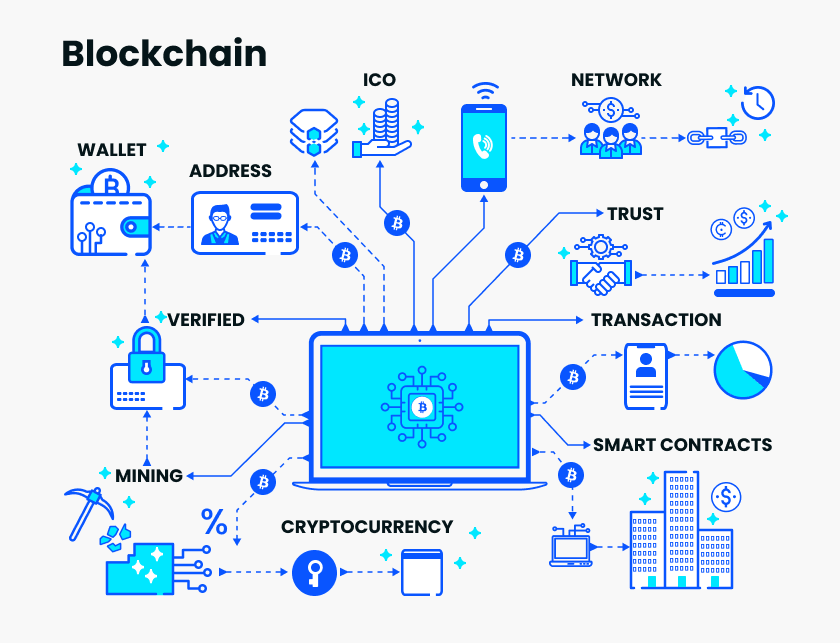
\includegraphics[width=0.66\textwidth]{Blockchain concepts.png}
    \caption[Blockchain concepts]{Key concepts of blockchain technology. Adapted from ...}
    \label{fig:blockchain_concepts}
\end{figure}

\subsection{Interacting with the Blockchain}
\label{subsec:interacting_with_the_blockchain}

A blockchain operates as a decentralized network of nodes, each maintaining a
copy of the entire blockchain. To interact with the blockchain, users send
transactions to the network, which are then validated and added to a block by
the nodes. This process requires a wallet—an application that allows users to
manage digital assets, interact with smart contracts, and send transactions.
Wallets provide a user-friendly interface for accessing the blockchain, signing
transactions with private keys, and viewing account balances and transaction
history.

Figure \ref{fig:how_does_a_blockchain_work} illustrates the steps involved in a
blockchain transaction. To execute a transaction, users must sign it with their
private key, proving ownership of the assets being transferred. The transaction
is then broadcast to the network, validated by participants, and added to a
block. Once confirmed, it becomes part of the immutable blockchain ledger,
accessible to all network participants.

This procedure is essential for altering the blockchain state; transactions
must be signed. In contrast, reading information from the blockchain requires
no signatures—users can simply query the network for the desired information.

\begin{figure}[H]
    \centering
    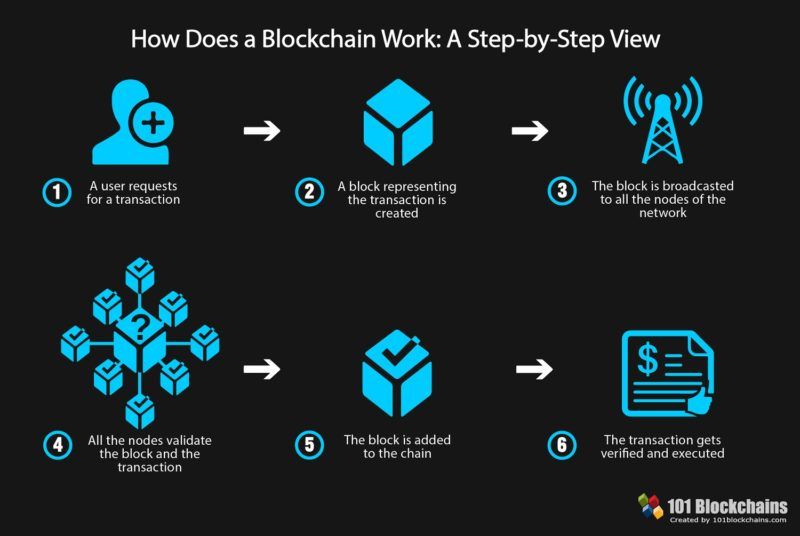
\includegraphics[width=0.66\textwidth]{How does a blockchain work.jpg}
    \caption[How does a blockchain work]{Overview of blockchain transaction processes. Extracted from ...}
    \label{fig:how_does_a_blockchain_work}
\end{figure}

\subsection{Blockchain}
\label{subsec:blockchain}

Blockchain is a decentralized and distributed ledger technology that enables
secure data recording and sharing across a network of computers. A blockchain
consists of a series of blocks, each containing a list of transactions. These
blocks are linked in a chronological and immutable chain, forming a transparent
and tamper-proof record. Key characteristics of blockchain technology include:

\paragraph{Decentralization:}
Blockchain operates on a decentralized network of nodes, eliminating a single
point of failure or control. Each node maintains a copy of the entire
blockchain.

\paragraph{Transparency:}
Data recorded on a blockchain is visible to all network participants, fostering
trust as users can independently verify transaction integrity without
intermediaries.

\paragraph{Immutability:}
Once recorded, transactions on a blockchain cannot be altered or deleted. This
is achieved through cryptographic techniques, ensuring a tamper-proof
historical record.

\paragraph{Security:}
Blockchain employs advanced cryptographic algorithms to secure transactions.
Network participants verify and validate transactions through consensus
mechanisms, preventing unauthorized changes.

\paragraph{Smart Contracts:}
Smart contracts are self-executing contracts with predefined rules encoded in
software. They automate transactions and enforce agreements without
intermediaries, enabling the creation of decentralized applications (DApps) on
blockchain networks.

Blockchain technology has applications across various industries, including
finance, supply chain management, healthcare, and decentralized finance (DeFi).
Its potential to enhance security, transparency, and efficiency has led to
widespread exploration of its capabilities. This ecosystem is often referred to
as Web3, a new paradigm for the internet aimed at decentralizing control and
empowering users with greater ownership and privacy over their data.

A compelling aspect of blockchain is how it harnesses human nature—greed and
self-interest—to create a secure and reliable system. Nodes are incentivized to
maintain blockchain integrity by earning cryptocurrency rewards, ensuring that
a majority of the network remains honest and cooperative, thus making the
system resistant to attacks.

\subsection{Wallets}
\label{subsec:wallets}

Cryptocurrency wallets utilize cryptographic principles to securely manage and
interact with digital assets on blockchain networks. Key cryptographic aspects
of wallets include:

\paragraph{Private and Public Keys:}
Wallets use a pair of cryptographic keys: a public key (wallet address) for
receiving funds and a private key for signing transactions. This relationship
is based on asymmetric cryptography, ensuring that only the rightful owner can
control their assets.

\paragraph{Digital Signatures:}
When initiating a transaction, it is digitally signed with the wallet's private
key, serving as proof of authorization. Digital signatures are generated using
cryptographic algorithms such as ECDSA or RSA, depending on the blockchain
protocol.

\paragraph{Hash Functions:}
Wallets use cryptographic hash functions to create unique representations of
transaction data, known as transaction hashes. These hashes verify transaction
integrity and prevent tampering.

\paragraph{Seed Phrases and Mnemonic Codes:}
Some wallets use mnemonic codes or seed phrases to back up access to funds if
the private key is lost. These phrases, generated from random words, serve as a
human-readable representation of the private key.

By leveraging these cryptographic techniques, wallets provide a secure means
for users to store, manage, and transact with digital assets, ensuring
confidentiality, integrity, and authenticity.

\subsection{Networks}
\label{subsec:networks}

Since Bitcoin's inception in 2009, blockchain technology has evolved
significantly, with numerous platforms emerging, each offering unique features.
Prominent networks in the decentralized ecosystem include:

\paragraph{Bitcoin (BTC):}
The first and most well-known cryptocurrency, Bitcoin was introduced by an
anonymous entity under the pseudonym Satoshi Nakamoto. It operates on a
decentralized network using a Proof of Work (PoW) consensus mechanism, designed
as a peer-to-peer electronic cash system.

\paragraph{Ethereum (ETH):}
Ethereum is a decentralized blockchain platform that enables the creation and
execution of smart contracts and DApps. Transitioning from a PoW to a Proof of
Stake (PoS) consensus model with the Ethereum 2.0 upgrade, it enhances
scalability and energy efficiency.

\paragraph{Polygon (MATIC):}
Polygon is a Layer 2 scaling solution for Ethereum that addresses scalability
issues by offering faster and cheaper transactions through sidechains.

\paragraph{Solana (SOL):}
Solana is designed for high-performance DApps and cryptocurrencies, using a
unique combination of Proof of History (PoH) and Proof of Stake (PoS) for high
throughput and low latency.

These examples highlight the diversity of blockchain networks, each with
distinct features and capabilities. As the ecosystem continues to evolve, new
technologies will emerge, expanding the possibilities for decentralized
applications and digital assets.

Many networks, like Ethereum and Polygon, are built using Solidity, allowing
compatibility with the Ethereum Virtual Machine (EVM). This enables developers
to deploy smart contracts across multiple networks using the same codebase,
enhancing reach and leveraging network effects. Other notable EVM-compatible
networks include Binance Smart Chain, Avalanche, Arbitrum, and Optimism.

\subsection{Smart Contracts}
\label{subsec:smart_contracts}

Smart contracts are self-executing contracts with terms encoded in software.
They automatically enforce agreements when predefined conditions are met,
eliminating the need for intermediaries. Key characteristics include:

\paragraph{Autonomy:}
Once deployed, smart contracts operate independently, executing transactions
without human intervention, ensuring impartial and transparent enforcement of
terms.

\paragraph{Trust:}
Smart contracts leverage blockchain's trustless nature, allowing parties to
rely on contract execution without a trusted third party, supported by the
decentralized and immutable nature of the blockchain.

\paragraph{Security:}
Due to blockchain's cryptographic principles, smart contracts are highly secure
and cannot be altered once deployed, providing reliability.

\paragraph{Efficiency:}
By automating execution, smart contracts reduce costs and processing times
associated with traditional contract enforcement, enhancing overall efficiency.

\paragraph{Versatility:}
Smart contracts can perform complex functions beyond simple transactions,
managing digital assets and interacting with other contracts, enabling diverse
DApp functionalities.

Smart contracts have applications across finance, supply chain management, real
estate, healthcare, and more. Their potential to revolutionize contract
execution in the digital age is significant.

\subsection{Token Standards}
\label{subsec:token_standards}

Token standards define the rules and functionalities of digital tokens on
blockchain networks, facilitating interoperability and usability. Key token
standards include ERC-20, ERC-721, and ERC-1155, as illustrated in Figure
\ref{fig:token_standards}.

\begin{figure}[H]
    \centering
    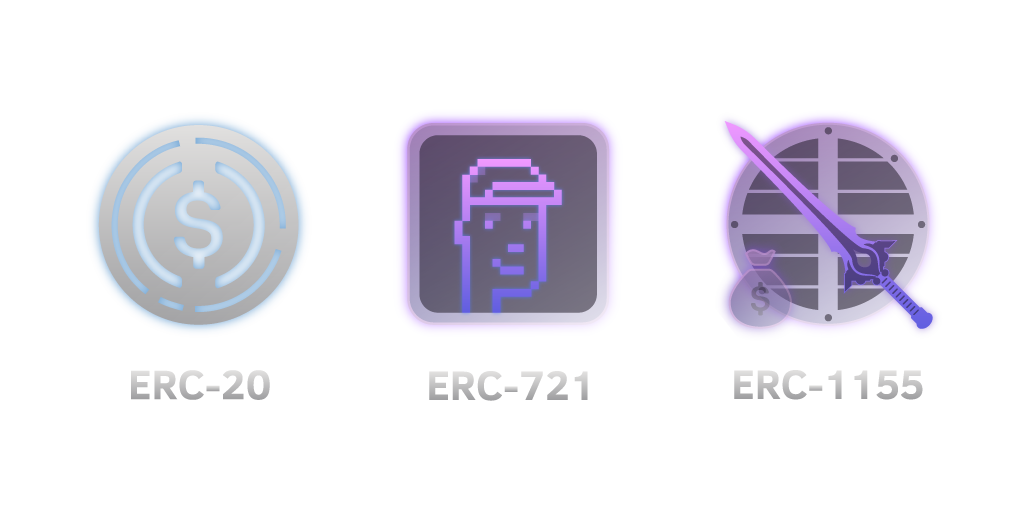
\includegraphics[width=0.66\textwidth]{Token standards.png}
    \caption[Token standards]{Overview of token standards. Extracted from ...}
    \label{fig:token_standards}
\end{figure}

\paragraph{ERC-20 (Ethereum Request for Comment 20):}
The most widely used token standard on Ethereum, ERC-20 governs fungible
tokens, allowing for seamless trading on exchanges. It includes functions for
transferring tokens and querying balances.

\paragraph{ERC-721 (Ethereum Request for Comment 721):}
This standard governs non-fungible tokens (NFTs), each of which is unique and
represents ownership of a specific asset. ERC-721 tokens are commonly used for
digital art and collectibles.

\paragraph{ERC-1155 (Ethereum Request for Comment 1155):}
This hybrid standard supports both fungible and non-fungible tokens within the
same contract, allowing efficient management of multiple token types and
reducing deployment costs.

These standards represent just a few examples shaping the landscape of
tokenization. As blockchain technology evolves, new standards will likely
emerge, driving further adoption across various industries.

\subsection{Non-Fungible Tokens (NFTs)}
\label{subsec:nfts}

In the context of event ticketing systems, NFTs offer great potential by
providing a secure and verifiable means of ticket issuance, transfer, and
validation. NFT-based tickets can incorporate unique metadata—such as event
details, seat numbers, and access permissions—creating a rich, customizable
experience for organizers and attendees. They can also be used to issue limited
edition or VIP tickets, granting exclusive access and additional benefits to
holders.
